\section{Durchführung}
\label{sec:Durchführung}

Die Reservoire der in Abb. \ref{fig:aufbau2} dargestellten Apparatur werden jeweils mit einer Wassermenge von 
\SI{}{\liter} aufgefüllt. Anschließend werden die Temperaturen $T1$ und $T2$ in den 
Reservoiren, die Drücke $p_a$ und $p_b$ im Verdampfungs- bzw. Verflüssigungsbereich und 
die Leistungsaufnahme des Kompressors gemessen. Der Zeittakt beträgt dabei eine Minute. 
Die Messung wird abgebrochen, sobald $T_1$ einen Wert von ca. $\SI{50}{\degrees\celsius}$ 
erreicht hat. 
\begin{figure}
    \centering
    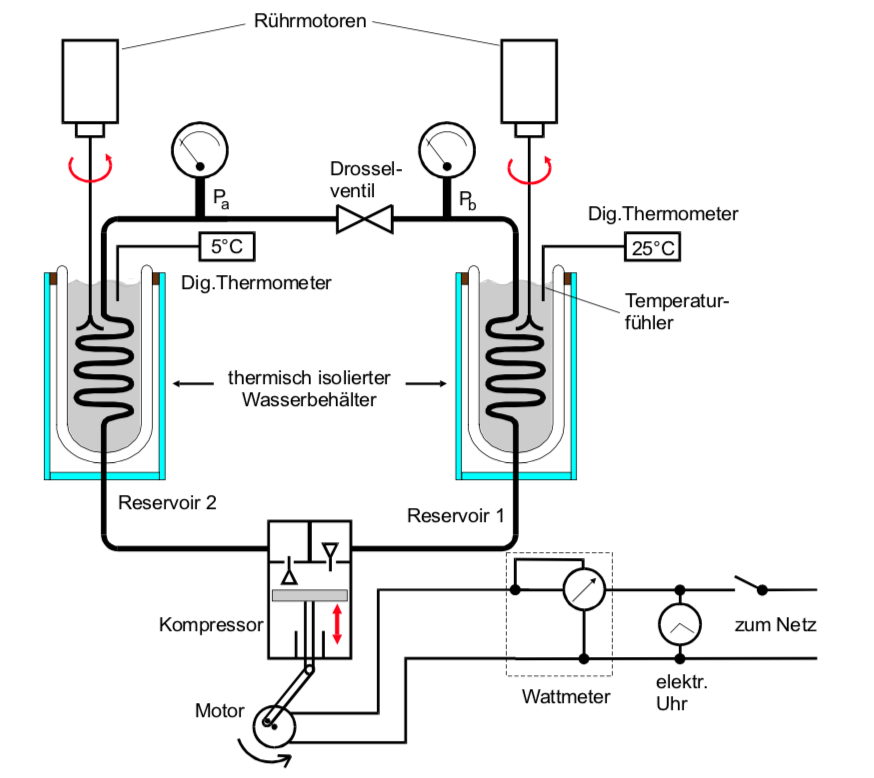
\includegraphics[width=10cm, height=10cm]{build/2.png}
    \caption{2}
    \label{fig:aufbau2}
\end{figure}